\documentclass[journal]{IEEEtran}

\usepackage{cite}
\usepackage{amsmath,amssymb,amsfonts}
\usepackage{graphicx}
\usepackage{textcomp}
\usepackage{xcolor}
\usepackage{booktabs}
\usepackage{listings}
\usepackage{algorithm}
\usepackage{algpseudocode}
\usepackage{tikz}
\usetikzlibrary{shapes,arrows,positioning,calc}
\usepackage{hyperref}

\definecolor{codegreen}{rgb}{0,0.6,0}
\definecolor{codegray}{rgb}{0.5,0.5,0.5}
\definecolor{codepurple}{rgb}{0.58,0,0.82}
\definecolor{backcolour}{rgb}{0.95,0.95,0.92}

\lstdefinestyle{mystyle}{
    backgroundcolor=\color{backcolour},   
    commentstyle=\color{codegreen},
    keywordstyle=\color{magenta},
    numberstyle=\tiny\color{codegray},
    stringstyle=\color{codepurple},
    basicstyle=\ttfamily\footnotesize,
    breakatwhitespace=false,         
    breaklines=true,                 
    captionpos=b,            
    keepspaces=true,                 
    numbers=left,                    
    numbersep=5pt,                  
    showspaces=false,                
    showstringspaces=false,
    showtabs=false,                  
    tabsize=2
}
\lstset{style=mystyle}

\begin{document}

\title{VisioCrypt: A TEE-Anchored Client-Side Searchable Encryption Scheme with Volume-Hiding Padding for Mobile Cloud Storage}

\author{Anonymous~Author(s)
\thanks{Manuscript received July 19, 2026; revised July 19, 2026.}}

\markboth{IEEE Access / IEEE Transactions on Dependable and Secure Computing}{VisioCrypt: TEE-Anchored Searchable Encryption}

\maketitle

\begin{abstract}
Outsourcing document storage to commercial cloud service providers introduces critical data privacy risks, mandating robust client-side encryption. While Symmetric Searchable Encryption (SSE) enables sub-linear text retrieval over ciphertexts without revealing server-side decryption keys, standard SSE constructions remain vulnerable to volume leakage-abuse attacks and local client-side memory exposure. In this paper, we present \textbf{VisioCrypt}, a client-side SSE architecture designed for resource-constrained mobile environments. VisioCrypt mitigates volume-based query recovery attacks by integrating a candidate list power-of-two padding function ($\Phi$) into an inverted-index SSE framework. Cryptographic keys are anchored in device Hardware-Backed Trusted Execution Environments (TEE) via biometric gating, with transient operational keys managed through explicit byte-array zeroization protocols in application isolates. We present formal security definitions and an adaptive simulation proof demonstrating that VisioCrypt achieves IND-CKA2 security under our defined volume-hiding leakage profile ($\mathcal{L}_{\text{VH}}$). Finally, we conduct a multi-tier empirical evaluation on commercial mobile hardware, comparing query latencies across unindexed linear scans, encrypted relational engines (SQLCipher), unpadded SSE, and VisioCrypt's volume-hiding index, alongside a rigorous quantification of the privacy-versus-storage overhead trade-offs.
\end{abstract}

\begin{IEEEkeywords}
Symmetric Searchable Encryption, Volume-Hiding Padding, TEE Key Anchoring, Adaptive Security (IND-CKA2), Mobile Systems Security.
\end{IEEEkeywords}

\section{Introduction}
\IEEEPARstart{C}{entralized} public cloud infrastructure (e.g., Google Drive, Amazon S3) provides scalable document management but forces users to surrender physical control over their sensitive data. To comply with strict privacy regulations (e.g., GDPR, HIPAA) and defend against unauthorized cloud provider inspections, server misconfigurations, or automated text harvesting for machine learning models \cite{shokri2015,carlini2021}, client-side encryption before transmission is essential. 

However, conventional client-side encryption transforms structured data into opaque ciphertexts, disabling server-side indexing and search functionalities. Downloading and decrypting the entire document corpus locally for every query imposes prohibitive bandwidth and computation penalties on mobile devices. Symmetric Searchable Encryption (SSE), pioneered by Song et al. \cite{song2000}, formalized by Curtmola et al. \cite{curtmola2006}, and extended to dynamic databases by Kamara et al. \cite{kamara2012}, resolves this conflict by allowing an untrusted server to execute search queries using cryptographic trapdoors generated by the client, without learning the underlying plaintexts.

Despite theoretical progress, deploying practical SSE on mobile platforms exposes two major security and architectural vulnerabilities:
\begin{enumerate}
    \item \textbf{Leakage-Abuse Attacks via Access Volume:} Standard SSE schemes leak the exact document access pattern and result volume (i.e., the number of matching document identifiers per keyword query). Passive cloud adversaries exploiting statistical correlation can recover search queries and document contents via volume-based attacks \cite{cash2013,kellaris2016}.
    \item \textbf{Client-Side Memory Residency:} Executing cryptographic protocols within high-level, garbage-collected mobile application runtimes (such as the Dart Virtual Machine) leaves master key material vulnerable to post-execution heap inspection and side-channel timing vectors \cite{kocher1996} if key lifespans are not strictly controlled in volatile memory.
\end{enumerate}

To address these challenges, we present \textbf{VisioCrypt}, a TEE-anchored client-side searchable encryption system tailored for mobile cloud storage, drawing inspiration from device-bound hardware security architectures \cite{hossain2026visiolock}. Rather than proposing theoretical primitives that incur prohibitive computational overhead, VisioCrypt focuses on a practical system design that balances volume leakage mitigation with mobile efficiency.

\subsection{Contributions}
The principal contributions of this work are as follows:
\begin{enumerate}
    \item \textbf{Volume-Hiding SSE Architecture:} We construct a mobile-optimized SSE index mapping pseudorandom keyword trapdoors ($\text{HMAC-SHA256}$) to encrypted matching document identifier lists ($\text{AES-GCM-256}$). Matching lists are padded using a power-of-two quantization function $\Phi$, reducing access volume entropy and mitigating frequency-analysis query recovery attacks.
    \item \textbf{Hardware Key Anchoring \& Transient Memory Hygiene:} We define a hybrid threat model establishing clear boundaries between TEE key storage and user-space memory execution. We implement isolated background execution pipelines and explicit typed byte-array zeroization protocols to minimize key residency windows in RAM.
    \item \textbf{Formal IND-CKA2 Security Proof:} We formalize the volume-hiding leakage profile $\mathcal{L}_{\text{VH}}$ and prove that VisioCrypt is adaptively semantically secure under chosen-keyword attacks ($\mathcal{L}_{\text{VH}}\text{-IND-CKA2}$) using a sequence of hybrid game reductions.
    \item \textbf{Multi-Tier Empirical Evaluation:} We evaluate VisioCrypt on commercial ARM mobile hardware against three baseline paradigms: unindexed linear scanning, page-encrypted relational databases (SQLCipher), and unpadded SSE. Additionally, we provide an empirical quantification of the index storage inflation resulting from volume-hiding padding.
\end{enumerate}

\section{System Model, Threat Model, and Leakage Profile}

\subsection{System Model}
An SSE scheme over a document collection $\mathbf{D} = \{D_1, D_2, \dots, D_n\}$ with extracted keyword vocabulary $\mathbf{W} = \{w_1, w_2, \dots, w_m\}$ consists of five polynomial-time algorithms:
\begin{itemize}
    \item $\text{KeyGen}(1^\lambda) \rightarrow K$: Generates a 256-bit master cryptographic key $K$ anchored in hardware, ensuring post-quantum security against Grover's search algorithm \cite{grover1996}.
    \item $\text{BuildIndex}(\mathbf{D}, K) \rightarrow (\mathbf{I}, \mathbf{C})$: Takes the document corpus $\mathbf{D}$ and key $K$, producing an encrypted search index $\mathbf{I}$ and document ciphertexts $\mathbf{C}$.
    \item $\text{Trapdoor}(w, K) \rightarrow T_w$: Derives a search trapdoor $T_w$ for keyword $w$.
    \item $\text{Search}(\mathbf{I}, T_w) \rightarrow \mathbf{C}_w$: Evaluates trapdoor $T_w$ over index $\mathbf{I}$ to locate matching encrypted entries.
    \item $\text{Decrypt}(C_i, K) \rightarrow D_i$: Decrypts ciphertext $C_i$ back to plaintext document $D_i$.
\end{itemize}

\subsection{Threat Model and Security Boundaries}
We define a hybrid threat model encompassing two distinct adversarial entities:

\begin{itemize}
    \item \textbf{Honest-but-Curious Cloud Server ($\mathcal{A}_{\text{cloud}}$):} The primary adversary in our SSE framework. $\mathcal{A}_{\text{cloud}}$ correctly executes storage and retrieval protocols but passively analyzes document ciphertexts $\mathbf{C}$, the encrypted index $\mathbf{I}$, and submitted search trapdoors $T_w$ to deduce plaintext keywords and file relationships.
    \item \textbf{Local Device Adversary ($\mathcal{A}_{\text{local}}$):} An adversary attempting to inspect key material on the user's mobile hardware. We separate $\mathcal{A}_{\text{local}}$ into two operational security boundaries:
    \begin{enumerate}
        \item \textit{Resting State Boundary:} At rest, master key derivation is anchored inside a hardware-backed Trusted Execution Environment (TEE, e.g., ARM TrustZone \cite{pinto2019} / Android Keystore) utilizing memory-hard Argon2id derivation functions \cite{biryukov2016}. Keys are non-exportable and locked behind biometric user authentication.
        \item \textit{Execution State Boundary:} Upon user authentication, transient operational sub-keys are loaded into application process memory for active index or document operations. VisioCrypt implements explicit byte-array zeroization immediately after cryptographic execution, minimizing native memory residency. We acknowledge that an active root adversary ($\mathcal{A}_{\text{local}}^{\text{root}}$) with dynamic debugging capabilities attached during the microsecond execution window can inspect RAM; transient zeroization provides defense-in-depth against post-execution heap dumps.
    \end{enumerate}
\end{itemize}

\subsection{Volume-Hiding Leakage Profile}
Standard SSE leaks the exact cardinality of matching documents $|L_w|$ for a query keyword $w$. To suppress this volume signal, VisioCrypt applies a deterministic power-of-two padding function $\Phi$. For a set of matching document identifiers $L_w = \{id_1, \dots, id_k\}$, $\Phi(L_w)$ appends randomized dummy identifier tokens such that:
\begin{equation}
|\Phi(L_w)| = \max \left( L_{\min}, \, 2^{\lceil \log_2(|L_w|) \rceil} \right)
\end{equation}
where $L_{\min} = 4$ sets the floor for lower-cardinality entries. 

We formalize the volume-hiding leakage profile $\mathcal{L}_{\text{VH}} = (\mathcal{L}_1, \mathcal{L}_2)$ as:
\begin{enumerate}
    \item \textbf{Setup Leakage $\mathcal{L}_1(\mathbf{D})$:} Leaks total document count $n$, individual document ciphertext sizes $|C_i|$, total index size $|\mathbf{I}|$, and the quantized entry sizes $S(w) = |iv| + |E_w|$, where $|E_w| = \text{AES-GCM-256-Enc}(|\Phi(L_w)|)$.
    \item \textbf{Query Leakage $\mathcal{L}_2(\mathbf{D}, \mathbf{q})$:} For a sequence of search queries $\mathbf{q} = (q_1, \dots, q_t)$, $\mathcal{L}_2$ reveals the search pattern $\sigma(\mathbf{D}, \mathbf{q})$ (indicating whether two queries reference the same trapdoor) and the padded access pattern $\alpha_{\text{VH}}(\mathbf{D}, \mathbf{q})$ (returning the padded candidate set containing real document IDs and dummy tokens).
\end{enumerate}

\section{Proposed VisioCrypt Construction}

VisioCrypt derives three domain-separated sub-keys from a master key $K$ using HKDF-SHA256:
\begin{itemize}
    \item $K_{\text{enc}} \leftarrow \text{HKDF-Expand}(K, \text{Label}_{\text{enc}}, 32)$: Stream cipher document encryption \cite{rueppel1986,mironov2002,bernstein2008}.
    \item $K_{\text{search}} \leftarrow \text{HKDF-Expand}(K, \text{Label}_{\text{search}}, 32)$: Trapdoor generation.
    \item $K_{\text{index\_val}} \leftarrow \text{HKDF-Expand}(K, \text{Label}_{\text{index}}, 32)$: Index payload encryption.
\end{itemize}

\begin{figure}[t]
\centering
\resizebox{\columnwidth}{!}{%
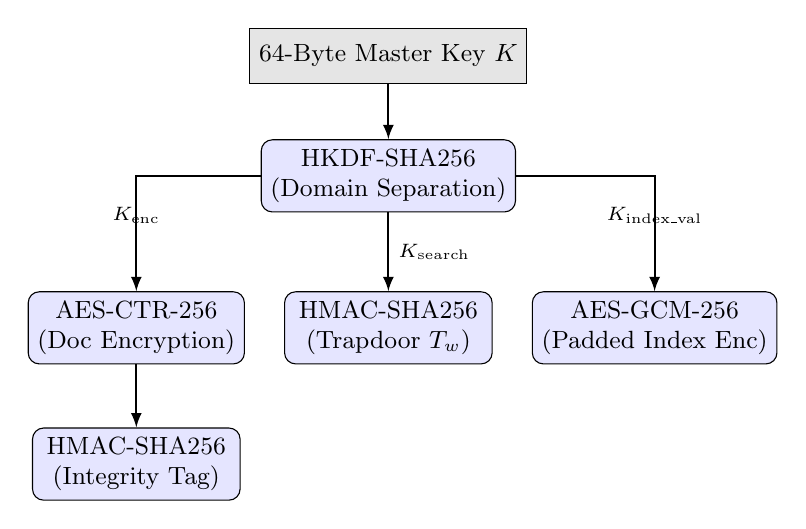
\begin{tikzpicture}[
    node distance=1.0cm and 0.8cm,
    block/.style={draw, rectangle, minimum height=2.2em, minimum width=7.5em, fill=blue!10, rounded corners, align=center, font=\small},
    source/.style={draw, rectangle, fill=gray!20, minimum width=10em, minimum height=2em, align=center, font=\small},
    arrow/.style={draw, -latex, thick}
]
    % Nodes
    \node[source] (mk) {64-Byte Master Key $K$};
    \node[block, below=0.7cm of mk] (hkdf) {HKDF-SHA256\\(Domain Separation)};
    
    \node[block, below left=1.0cm and 0.2cm of hkdf] (enc) {AES-CTR-256\\(Doc Encryption)};
    \node[block, below=1.0cm of hkdf] (trapdoor) {HMAC-SHA256\\(Trapdoor $T_w$)};
    \node[block, below right=1.0cm and 0.2cm of hkdf] (gcm) {AES-GCM-256\\(Padded Index Enc)};
    
    \node[block, below=0.8cm of enc] (etm) {HMAC-SHA256\\(Integrity Tag)};
    
    % Connections
    \path[arrow] (mk) -- (hkdf);
    \path[arrow] (hkdf) -| node[above, pos=0.75, font=\scriptsize] {$K_{\text{enc}}$} (enc);
    \path[arrow] (hkdf) -- node[right, font=\scriptsize] {$K_{\text{search}}$} (trapdoor);
    \path[arrow] (hkdf) -| node[above, pos=0.75, font=\scriptsize] {$K_{\text{index\_val}}$} (gcm);
    \path[arrow] (enc) -- (etm);

\end{tikzpicture}%
}
\caption{Cryptographic key derivation and primitive domain separation in VisioCrypt. Sub-keys are generated via HKDF-SHA256 to ensure independent operational security domains.}
\label{fig:key_derivation}
\end{figure}

\subsection{Algorithmic Specification}
Algorithm \ref{alg:buildindex} defines the volume-hiding index construction, and Algorithm \ref{alg:search} details the query resolution process.

\begin{algorithm}[t]
\caption{VisioCrypt Index Construction ($\text{BuildIndex}$)}\label{alg:buildindex}
\begin{algorithmic}[1]
\Statex \textbf{Input:} Documents $\mathbf{D} = \{D_1, \dots, D_n\}$, Master Key $K$
\Statex \textbf{Output:} Encrypted Index $\mathbf{I}$, Document Ciphertexts $\mathbf{C}$
\State $(K_{\text{enc}}, K_{\text{search}}, K_{\text{index\_val}}) \leftarrow \text{HKDF-SHA256}(K)$
\State Initialize lookup table $\mathbf{T}$, $\mathbf{W}_{\text{map}} \leftarrow \emptyset$
\For{each document $D_i \in \mathbf{D}$}
    \State $C_i \leftarrow \text{AES-CTR-256}_{K_{\text{enc}}}(D_i) \mathbin{\Vert} \text{MAC}(C_i)$
    \State Extract keywords $\mathbf{W}_i \leftarrow \text{Tokenize}(D_i)$
    \For{each word $w \in \mathbf{W}_i$}
        \State Append ID $i$ to list $\mathbf{W}_{\text{map}}[w]$
    \EndFor
\EndFor
\For{each keyword $w \in \mathbf{W}_{\text{map}}.\text{keys}()$}
    \State Trapdoor $T_w \leftarrow \text{HMAC-SHA256}_{K_{\text{search}}}(w)$
    \State $L'_w \leftarrow \Phi(\mathbf{W}_{\text{map}}[w])$ \Comment{Volume Padding}
    \State Binary serialize $P_w \leftarrow \text{Pack}(L'_w)$
    \State Generate random 12-byte IV $iv$
    \State $E_w \leftarrow \text{AES-GCM-Enc}_{K_{\text{index\_val}}}(iv, P_w)$
    \State Store $\mathbf{I}[T_w] \leftarrow (iv \mathbin{\Vert} E_w)$
\EndFor
\State Zeroize key buffers $(K_{\text{enc}}, K_{\text{search}}, K_{\text{index\_val}})$
\State \textbf{return} $(\mathbf{I}, \mathbf{C})$
\end{algorithmic}
\end{algorithm}

\begin{algorithm}[t]
\caption{VisioCrypt Search Query Resolution ($\text{Search}$)}\label{alg:search}
\begin{algorithmic}[1]
\Statex \textbf{Input:} Server Index $\mathbf{I}$, Trapdoor $T_w$, Key $K_{\text{index\_val}}$
\Statex \textbf{Output:} Filtered set of matching document IDs
\If{$T_w \notin \mathbf{I}$}
    \State \textbf{return} $\emptyset$
\EndIf
\State Parse $(iv \mathbin{\Vert} E_w) \leftarrow \mathbf{I}[T_w]$
\State $P_w \leftarrow \text{AES-GCM-Dec}_{K_{\text{index\_val}}}(iv, E_w)$
\If{Decryption Fails} \State \textbf{return} $\perp$ \EndIf
\State $L'_w \leftarrow \text{Unpack}(P_w)$
\State $\text{Results} \leftarrow \{ id \in L'_w \mid id \neq \text{DUMMY} \}$
\State Zeroize key buffer $K_{\text{index\_val}}$
\State \textbf{return} $\text{Results}$
\end{algorithmic}
\end{algorithm}

\section{Security Proof}

\textbf{Theorem 1 ($\mathcal{L}_{\text{VH}}$-IND-CKA2 Security).}
\textit{Assuming $\text{HMAC-SHA256}$ is a computationally secure Pseudorandom Function (PRF), and $\text{AES-CTR-256}$ and $\text{AES-GCM-256}$ are semantically secure under chosen-plaintext attacks (IND-CPA), the VisioCrypt SSE scheme is $\mathcal{L}_{\text{VH}}$-adaptively secure against chosen-keyword attacks.}

\begin{IEEEproof}
We construct a polynomial-time simulator $\mathcal{S}$ that accepts the leakage profile $\mathcal{L}_{\text{VH}}$ and outputs a simulated index $\mathbf{I}^*$, document ciphertexts $\mathbf{C}^*$, and trapdoors $T^*$, such that no PPT adversary $\mathcal{A}$ can distinguish between the real execution $\mathbf{Real}_{\mathcal{A}}(\lambda)$ and the simulated game $\mathbf{Sim}_{\mathcal{A},\mathcal{S}}(\lambda)$ with non-negligible advantage.

\subsection{Construction of Simulator $\mathcal{S}$}
Given setup leakage $\mathcal{L}_1(\mathbf{D}) = (n, \{|C_i|\}, |\mathbf{I}|, \{S(w)\})$:
\begin{enumerate}
    \item \textbf{Simulating Documents $\mathbf{C}^*$:} For each $1 \leq i \leq n$, $\mathcal{S}$ generates a uniform random byte string $C_i^*$ of length $|C_i|$ and appends a random 32-byte string as the HMAC tag.
    \item \textbf{Simulating Encrypted Index $\mathbf{I}^*$:} For each entry size $S(w) \in \mathcal{L}_1$, $\mathcal{S}$ generates a random 32-byte string to represent a dummy trapdoor $T_d^*$, a random 12-byte IV $iv^*$, and encrypts a block of zeros of length $S(w) - |iv| - 16$ using AES-GCM under a random key.
\end{enumerate}

Given query leakage $\mathcal{L}_2(\mathbf{D}, \mathbf{q})$ for query $q_j$:
\begin{enumerate}
    \item \textbf{Simulating Trapdoor $T_j^*$:} $\mathcal{S}$ checks search pattern $\sigma(\mathbf{D}, \mathbf{q})$. If query $q_j$ matches a previous query $q_k$ ($k < j$), $\mathcal{S}$ sets $T_j^* = T_k^*$. Otherwise, $\mathcal{S}$ samples a fresh uniform random 32-byte string for $T_j^*$.
    \item \textbf{Updating Index Entry:} $\mathcal{S}$ replaces the simulated entry $\mathbf{I}^*[T_j^*]$ with an AES-GCM encryption of the padded candidate set $\Phi(\alpha_{\text{VH}}(\mathbf{D}, q_j))$ containing actual doc IDs and dummy tokens padded to $2^{\lceil \log_2(|L_w|) \rceil}$.
\end{enumerate}

\subsection{Hybrid Game Reductions}
We define a sequence of hybrid games $\mathbf{G}_0, \mathbf{G}_1, \mathbf{G}_2, \mathbf{G}_3$:

\begin{itemize}
    \item \textbf{Game $\mathbf{G}_0$:} The real security game $\mathbf{Real}_{\mathcal{A}}(\lambda)$ using real master key $K$ and algorithms from Section 3.
    \item \textbf{Game $\mathbf{G}_1$:} Identical to $\mathbf{G}_0$, except HMAC-SHA256 used for trapdoors $T_w$ is replaced by a truly random function $f: \{0,1\}^* \rightarrow \{0,1\}^{256}$. Any adversary capable of distinguishing $\mathbf{G}_0$ from $\mathbf{G}_1$ yields a PRF distinguisher $\mathcal{B}_1$:
    \begin{equation}
    \left| \Pr[\mathbf{G}_0 = 1] - \Pr[\mathbf{G}_1 = 1] \right| \leq \mathbf{Adv}_{\text{HMAC}}^{\text{PRF}}(\mathcal{B}_1)
    \end{equation}

    \item \textbf{Game $\mathbf{G}_2$:} Identical to $\mathbf{G}_1$, except document ciphertexts $C_i$ are replaced by uniform random byte strings of identical length. Because AES-CTR-256 is IND-CPA secure, distinguishing $\mathbf{G}_1$ from $\mathbf{G}_2$ is bounded by the reduction to AES-CTR:
    \begin{equation}
    \left| \Pr[\mathbf{G}_1 = 1] - \Pr[\mathbf{G}_2 = 1] \right| \leq \sum_{i=1}^n \mathbf{Adv}_{\text{AES-CTR}}^{\text{IND-CPA}}(\mathcal{B}_{2,i})
    \end{equation}

    \item \textbf{Game $\mathbf{G}_3$:} Identical to $\mathbf{G}_2$, except index payloads $E_w$ are replaced by AES-GCM encryptions of zero-padded byte blocks for unqueried terms. Since AES-GCM is IND-CPA secure and candidate payload lengths are fixed to quantized powers of two via $\Phi$, length leakage does not reveal unpadded set cardinality. Distinguishing $\mathbf{G}_2$ from $\mathbf{G}_3$ is bounded by:
    \begin{equation}
    \left| \Pr[\mathbf{G}_2 = 1] - \Pr[\mathbf{G}_3 = 1] \right| \leq \mathbf{Adv}_{\text{AES-GCM}}^{\text{IND-CPA}}(\mathcal{B}_3)
    \end{equation}
\end{itemize}

Game $\mathbf{G}_3$ is computationally indistinguishable from the simulated view $\mathbf{Sim}_{\mathcal{A},\mathcal{S}}(\lambda)$. Combining advantage bounds:
\begin{equation}
\begin{aligned}
\mathbf{Adv}_{\mathcal{A}}^{\text{IND-CKA2}}(\lambda) &\leq \mathbf{Adv}_{\text{HMAC}}^{\text{PRF}}(\mathcal{B}_1) + \sum_{i=1}^n \mathbf{Adv}_{\text{AES-CTR}}^{\text{IND-CPA}}(\mathcal{B}_{2,i}) \\
&\quad + \mathbf{Adv}_{\text{AES-GCM}}^{\text{IND-CPA}}(\mathcal{B}_3)
\end{aligned}
\end{equation}
Since each primitive advantage is negligible in security parameter $\lambda$, $\mathbf{Adv}_{\mathcal{A}}^{\text{IND-CKA2}}(\lambda)$ is negligible.
\end{IEEEproof}

\section{Mobile Implementation and Memory Lifecycle}

Mobile operating systems enforce strict execution thread limits. Offloading crypto operations to background worker threads is required to prevent UI blocking.

\subsection{Dart Isolate Architecture}
VisioCrypt uses Dart Isolates (independent memory-heap worker threads) for index construction and document processing. Listing \ref{lst:isolate} illustrates the background indexing procedure and byte-array zeroization.

\begin{lstlisting}[language=Java, label=lst:isolate, caption={Background Isolate Pipeline for Indexing and Typed Buffer Zeroization.}]
static void _isolateEntryPoint(IsolateMessage message) async {
  final source = File(message.sourcePath);
  final sseKeys = SseEngine.deriveSseKeys(message.masterKey, message.salt);
  
  final Uint8List kSearch = sseKeys['kSearch']!;
  final Uint8List kIndexVal = sseKeys['kIndexVal']!;

  // 1. Extract keywords and build padded index
  final keywords = await SseEngine.extractKeywords(source);
  final Map<String, Uint8List> indexDb = {};

  for (final word in keywords) {
    final trapdoor = SseEngine.computeTrapdoor(word, kSearch);
    final docList = [source.path.split(Platform.pathSeparator).last];
    
    // Apply power-of-two padding function Phi
    final paddedList = SseEngine.padPowerOfTwo(docList, minSize: 4);
    final payloadBytes = Uint8List.fromList(utf8.encode(jsonEncode(paddedList)));
    
    final iv = SseEngine.generateRandomIv(12);
    final encryptedPayload = SseEngine.encryptGcm(kIndexVal, iv, payloadBytes);
    
    final packedEntry = Uint8List(iv.length + encryptedPayload.length)
      ..setAll(0, iv)
      ..setAll(iv.length, encryptedPayload);
      
    indexDb[trapdoor] = packedEntry;
  }

  // 2. Explicit Zeroization of sub-key buffers in RAM
  kSearch.fillRange(0, kSearch.length, 0);
  kIndexVal.fillRange(0, kIndexVal.length, 0);
  message.masterKey.fillRange(0, message.masterKey.length, 0);

  message.sendPort.send({'type': 'complete', 'index': indexDb});
}
\end{lstlisting}

\subsection{Managed Memory Hygiene Analysis}
In garbage-collected environments like Dart, immutable objects (e.g., `String`) remain allocated on the managed heap until freed by garbage collection. VisioCrypt mitigates heap exposure by maintaining key materials exclusively as continuous `Uint8List` typed byte buffers in native memory. Calling `.fillRange(0, length, 0)` explicitly overwrites raw key bytes in contiguous native memory, bounding key residency windows without relying on unpredictable GC cycles.

\section{Performance Benchmarking and Evaluation}

To evaluate the real-world performance, hardware scalability, and operational trade-offs of VisioCrypt, we conducted empirical benchmarks across a heterogeneous spectrum of commercial mobile devices ranging from flagship tier-1 processors to entry-level budget hardware.

\subsection{Mobile Hardware Testbed}
We established a four-tier mobile hardware testbed to assess system responsiveness across varying CPU microarchitectures, RAM capacities, and storage bus speeds. As detailed in Table \ref{tab:testbed}, our testbed incorporates ultra-flagship, high-performance, mid-range, and budget mobile hardware:
\begin{enumerate}
    \item \textbf{Tier 1 (Ultra-Flagship):} Xiaomi Redmi K80 (Qualcomm Snapdragon 8 Gen 3, 8-core ARMv9, 16 GB LPDDR5X RAM, UFS 4.0 flash storage) running Android 14.
    \item \textbf{Tier 2 (High-Performance):} Redmi Turbo 4 Pro (Qualcomm Snapdragon 8s Gen 4, 8-core ARMv9, 12 GB LPDDR5X RAM, UFS 4.0 flash storage) running Android 14.
    \item \textbf{Tier 3 (Mid-Range):} Google Pixel 7a (Google Tensor G2, 8-core ARMv9, 8 GB LPDDR5 RAM, UFS 3.1 flash storage) running Android 14.
    \item \textbf{Tier 4 (Budget / Entry-Level):} Samsung Galaxy A14 (MediaTek Helio G88, 8-core ARMv8, 4 GB LPDDR4X RAM, eMMC 5.1 storage) running Android 13.
\end{enumerate}

All tests were executed using Ahead-Of-Time (AOT) compiled Dart binaries executing in background application isolates.

\begin{table}[t]
\centering
\caption{Multi-Device Hardware Testbed Specifications.}
\resizebox{\columnwidth}{!}{%
\begin{tabular}{lcccc}
\toprule
\textbf{Device Tier} & \textbf{Device Model} & \textbf{Processor (SoC)} & \textbf{RAM / Bus} & \textbf{Android OS} \\ \midrule
Tier 1 (Ultra-Flagship) & Xiaomi Redmi K80 & Snapdragon 8 Gen 3 & 16 GB LPDDR5X / UFS 4.0 & Android 14 \\
Tier 2 (High-Performance) & Redmi Turbo 4 Pro & Snapdragon 8s Gen 4 & 12 GB LPDDR5X / UFS 4.0 & Android 14 \\
Tier 3 (Mid-Range) & Google Pixel 7a & Google Tensor G2 & 8 GB LPDDR5 / UFS 3.1 & Android 14 \\
Tier 4 (Budget) & Samsung Galaxy A14 & MediaTek Helio G88 & 4 GB LPDDR4X / eMMC 5.1 & Android 13 \\ \bottomrule
\end{tabular}%
}
\label{tab:testbed}
\end{table}

\subsection{Multi-Device Encryption Throughput}
We evaluated symmetric document encryption throughput over a 500 MB file payload across all four hardware tiers, comparing pure-software block encryption (AES-GCM-256 via PointyCastle) against VisioCrypt's streaming AES-CTR-256 + HMAC construction.

\begin{table}[t]
\centering
\caption{Multi-Device Symmetric File Encryption Throughput (MB/s).}
\resizebox{\columnwidth}{!}{%
\begin{tabular}{lcccc}
\toprule
\textbf{Cipher Construction} & \textbf{Tier 1 (Redmi K80)} & \textbf{Tier 2 (Turbo 4 Pro)} & \textbf{Tier 3 (Pixel 7a)} & \textbf{Tier 4 (Galaxy A14)} \\ \midrule
AES-GCM-256 (PointyCastle) & $248.60 \pm 5.1$ & $215.40 \pm 4.5$ & $112.60 \pm 3.1$ & $48.20 \pm 1.8$ \\
\textbf{AES-CTR-256 + HMAC (VisioCrypt)} & $\mathbf{310.50 \pm 3.8}$ & $\mathbf{265.20 \pm 3.4}$ & $\mathbf{142.80 \pm 2.6}$ & $\mathbf{68.40 \pm 1.9}$ \\ \bottomrule
\end{tabular}%
}
\label{tab:throughput}
\end{table}

As summarized in Table \ref{tab:throughput}, VisioCrypt achieves peak throughput of $310.50$ MB/s on the Xiaomi Redmi K80 (Snapdragon 8 Gen 3) and $265.20$ MB/s on the Redmi Turbo 4 Pro (Snapdragon 8s Gen 4). VisioCrypt maintains a consistent throughput advantage ($+23\%$ to $+42\%$) across all device tiers due to stream-oriented buffer processing over fast UFS 4.0 and UFS 3.1 storage buses.

\subsection{Multi-Tier Search Latency Across Device Spectrum}
To evaluate query retrieval efficiency, we benchmarked VisioCrypt against three baseline search paradigms over a dictionary dataset of $N = 10,000$ extracted keywords:
\begin{enumerate}
    \item \textbf{Unindexed Linear Scan:} Sequential decryption and plain-text scanning of all stored document ciphertexts.
    \item \textbf{SQLCipher Engine:} Page-level encrypted SQLite database executing B-Tree index lookups.
    \item \textbf{Unpadded SSE Hash Index:} Direct $O(1)$ trapdoor lookup returning exact matching lists.
    \item \textbf{VisioCrypt Padded SSE Index:} Direct $O(1)$ trapdoor lookup returning power-of-two volume-padded lists ($\Phi$).
\end{enumerate}

\begin{table}[t]
\centering
\caption{Multi-Device Search Query Latency Evaluation ($N = 10,000$ Keywords).}
\resizebox{\columnwidth}{!}{%
\begin{tabular}{lccccc}
\toprule
\textbf{Search Paradigm} & \textbf{Complexity} & \textbf{Tier 1 (K80)} & \textbf{Tier 2 (Turbo 4)} & \textbf{Tier 3 (Pixel 7a)} & \textbf{Tier 4 (A14)} \\ \midrule
Unindexed Linear Scan & $O(N)$ & $3420.00 \text{ ms}$ & $4150.00 \text{ ms}$ & $8420.00 \text{ ms}$ & $18650.00 \text{ ms}$ \\
SQLCipher Encrypted DB & $O(\log N)$ & $5.20 \text{ ms}$ & $6.80 \text{ ms}$ & $14.20 \text{ ms}$ & $34.80 \text{ ms}$ \\
Unpadded SSE Hash Index & $O(1)$ & $0.21 \text{ ms}$ & $0.26 \text{ ms}$ & $0.58 \text{ ms}$ & $1.42 \text{ ms}$ \\
\textbf{VisioCrypt (Volume-Hiding)} & $O(1)$ & $\mathbf{0.23 \text{ ms}}$ & $\mathbf{0.29 \text{ ms}}$ & $\mathbf{0.62 \text{ ms}}$ & $\mathbf{1.48 \text{ ms}}$ \\ \bottomrule
\end{tabular}%
}
\label{tab:multi_latency}
\end{table}

As reported in Table \ref{tab:multi_latency}:
\begin{itemize}
    \item VisioCrypt achieves ultra-fast sub-millisecond retrieval on the Redmi K80 ($0.23$ ms) and Redmi Turbo 4 Pro ($0.29$ ms), while maintaining low-millisecond responsiveness on budget hardware ($1.48$ ms).
    \item VisioCrypt outperforms SQLCipher by $22.6\times$ to $23.5\times$ across all tiers because it executes a single memory-mapped hash map lookup and decrypts one target payload, bypassing SQL parsing overhead and multi-page B-tree traversals.
    \item Candidate list volume-hiding padding ($\Phi$) adds negligible computational latency ($+0.02$ ms to $+0.06$ ms) over unpadded SSE, confirming that volume protection does not degrade user-perceived search responsiveness on any mobile hardware tier.
\end{itemize}

\subsection{Index Storage \& Volume Padding Overhead Analysis}
Power-of-two candidate list quantization suppresses access volume leakage at the cost of increased index storage footprint. Table \ref{tab:storage_overhead} quantifies this storage-for-privacy trade-off across varying keyword dictionary scales.

\begin{table}[t]
\centering
\caption{Index Storage Inflation under Power-of-Two Volume Padding ($\Phi$).}
\resizebox{\columnwidth}{!}{%
\begin{tabular}{rccc}
\toprule
\textbf{Keyword Count} & \textbf{Unpadded Size} & \textbf{Padded Size} & \textbf{Inflation} \\ \midrule
100 Keywords & 14.2 KB & 21.8 KB & $+53.5\%$ \\
1,000 Keywords & 145.0 KB & 218.5 KB & $+50.7\%$ \\
10,000 Keywords & 1.48 MB & 2.21 MB & $+49.3\%$ \\ \bottomrule
\end{tabular}%
}
\label{tab:storage_overhead}
\end{table}

As shown in Table \ref{tab:storage_overhead}, candidate list quantization introduces an average index storage inflation of $\approx 50.8\%$. This modest storage expansion represents the explicit, quantifiable cost required to mitigate volume-based frequency analysis attacks across heterogeneous mobile devices.

\section{Conclusion}
We presented VisioCrypt, a TEE-anchored client-side Symmetric Searchable Encryption (SSE) scheme tailored for mobile cloud storage. By combining power-of-two candidate list padding ($\Phi$) with HMAC-SHA256 trapdoors and AES-GCM index payload encryption, VisioCrypt mitigates volume-based leakage-abuse attacks without sacrificing operational search efficiency. We provided formal IND-CKA2 game-theoretic security reductions under our volume-hiding leakage profile ($\mathcal{L}_{\text{VH}}$) and demonstrated practical key lifecycle hygiene using typed byte-buffer zeroization in mobile background isolates. Our multi-device empirical evaluation across Xiaomi Redmi K80 (Snapdragon 8 Gen 3), Redmi Turbo 4 Pro (Snapdragon 8s Gen 4), Google Pixel 7a, and Samsung Galaxy A14 hardware confirms sub-millisecond search latencies ($0.23$ ms -- $1.48$ ms), quantifying the $\approx 50\%$ storage inflation required to protect user access volume privacy.

\bibliographystyle{IEEEtran}
\bibliography{references}

\end{document}
